% In this file you should put the actual content of the blueprint.
% It will be used both by the web and the print version.
% It should *not* include the \begin{document}
%
% If you want to split the blueprint content into several files then
% the current file can be a simple sequence of \input. Otherwise It
% can start with a \section or \chapter for instance.

\section{Introduction}

The purpose of this paper is to report on the \emph{Equational Theories Project} (ETP)\footnote{\url{https://teorth.github.io/equational_theories/}}, a pilot project launched\footnote{\url{https://terrytao.wordpress.com/2024/09/25}} in September 2024 to explore new ways to collaboratively work on mathematical research projects using machine assistance. The project goal, in the area of universal algebra, was selected to be particularly amenable to crowdsourced and computer-assisted techniques, while still being of mathematical research interest. \note{Describe outcomes}

\subsection{Magmas and Equational Laws}

In order to describe the mathematical goals of the ETP, we need some notation. A \emph{magma} $M = (M,\op)$ is a set $M$ (known as the \emph{carrier}) together with a binary operation $\op \colon M \times M \to M$. An \emph{equational law} for a magma, or \emph{law} for short, is an identity involving $\op$ and some formal indeterminates, which we will typically denote using the Roman letters $\x,\y,\z,\w,\uu,\vv$, as well as the formal equality symbol $\formaleq$ in place of the equality symbol $=$ to emphasize the formal nature of the law.

In the ETP, a unique number was assigned to each equational law, via a numbering system that we describe in \Cref{numbering-app}.  For instance, the \emph{commutative law} $\x \op \y \formaleq \y \op \x$ is assigned the equation number \Cref{eq43}, while the \emph{associative law} $(\x \op \y) \op \z \formaleq \x \op (\y \op \z)$ is assigned the equation number \Cref{eq4512}.  A list of all equations referred to by number in this paper is provided in \Cref{numbering-app}.

A magma $M$ obeys a law $E$ if the law $E$ holds for all possible assignments of the indeterminate to $M$, in which case we write $M \models E$. Thus for instance $M \models E43$ if one has $x \op y = y \op x$ for all $x,y \in M$.

We say that a law $E$ \emph{entails} or \emph{implies} another law $E'$ if every magma that obeys $E$, also implies $E'$: $(M \models E) \implies (M \models E')$.  We write this relation as $E \vdash E'$. We say that two laws are \emph{equivalent} if they entail each other. For instance, the constant law $\x \op \y \formaleq \z \op \w$ \Cref{eq46} can easily be seen to be equivalent to the law $\x \op \x \formaleq \y \op \z$ \Cref{eq41}.  It is easy to see that $\vdash$ is a pre-order, that is to say a partial order after one quotients by equivalence.

In this entailment pre-ordering, the maximal element is given by the trivial law $\x\formaleq\x$ \Cref{eq1}, and the minimal element is given by the singleton law $\x\formaleq \y$ \Cref{eq2}, thus $E2 \vdash E \vdash E1$ for all laws $E$.

The \emph{order} of an equational law is the number of occurrences of the magma operation. For instance, the commutative law \Cref{eq43} has order $2$, while the associative law \Cref{eq4512} has order $4$. We note some selected laws of small order that have previously appeared in the literature:
\begin{itemize}
\item The \emph{central groupoid law} $\x \formaleq (\y \op \x) \op (\x \op \z)$ \Cref{eq168} is an order $3$ law introduced by Evans \cite{evans} and studied further by Knuth \cite{knuth} and many further authors, being closely related to central digraphs (also known as unique path property diagraphs), and leading in particular to the discovery of the Knuth-Bendix algorithm \cite{knuth-bendix}; see \cite{klt} for a more recent survey.
\item \emph{Tarski's axiom} $\x \formaleq \y \op ( (\z \op (\x \op (\y \op \z))))$ \Cref{eq543} is an order $4$ law that was shown by Tarski \cite{Tarski1938} to characterize the operation of subtraction in an abelian group; that is to say, a magma $M$ obeys \Cref{eq543} if and only if there is an abelian group structure on $M$ for which $x \op y = x-y$ for all $x,y \in M$.
\item In a similar vein, it was shown in \cite{mendelsohn-padmanabhan} (see also \cite{meredith-prior}) that the order $4$ law
$\x \formaleq (\y \op \z) \op (\y \op (\x \op \z))$ \Cref{eq1571} characterizes addition (or subtraction) in an abelian group of exponent $2$; it was shown in \cite{mccune_et_al} that the order $4$ law $\x \formaleq (\y \op ((\x \op \y) \op \y)) \op (\x \op (\z \op \y))$ \Cref{eq345169} characterizes the Sheffer stroke in a boolean algebra, and it was shown in \cite{higman-neumann} that the order $8$ law
$\x \formaleq \y \op ((((\y \op \y) \op \x) \op \z) \op (((\y \op \y) \op \y) \op \z))$ \Cref{eq42323216} characterizes division in a (not necessarily abelian) group.
\end{itemize}
Some further examples of laws characterizing well-known algebraic structures are listed in \cite{mccune-survey}.

The Birkhoff completeness theorem \cite[Th. 3.5.14]{term-rewriting} implies that an implication $E \vdash E'$ of equational laws holds if and only if the left-hand side of $E'$ can be transformed into the right-hand side by a finite number of substitution rewrites using the law $E$. However, the problem of determining whether such an implication holds is undecidable in general \cite{mckenzie}. Even when the order is small, some implications\footnote{Another contemporaneous example of this phenomenon was the solution of the Robbins problem \cite{robbins}.} can require lengthy computer-assisted proofs; for instance, it was noted in \cite{Kisielewicz2} that the order $4$ law $\x \formaleq (\y \op \x) \op ((\x \op \z) \op \z)$ \Cref{eq1689} was equivalent to the singleton law \Cref{eq2}, but all known proofs are computer-assisted.

\subsection{The Equational Theories Project}

As noted in \Cref{numbering-app}, there are $4694$ equational laws of order at most $4$. The primary mathematical goal of the ETP was to completely determine the \emph{implication graph} for these laws, in which there is a directed edge from $E$ to $E'$ precisely when $E \vdash E'$. Such systematic determinations of implication graphs have been seen previously in the literature; for instance, in \cite{phillips-vojtechovsky}, the relations between $60$ identities of Bol--Moufang type were established, and in the blog post \cite[\S 17]{Wolfram_2022}, some initial steps towards generating this graph for the first hundred or so laws on our list were performed. However, to our knowledge, the ETP is the first project to study such implications at the scale of thousands of laws.

The ETP requires the determination of the truth or falsity of $4694^2 = 22033636$ implications; while one can use properties such as the transitivity of entailment to reduce the work somewhat, this is clearly a task that requires significant automation. It was also a project highly amenable to crowdsourcing, in which different participants could work on developing different techniques, each of which could be used to fill out a different part of the implication graph. In this respect, the project could be compared with a Polymath project \cite{Gowers2009}, which used online forums such as blogs and wikis to openly collaborate on a mathematical research problem. However, the Polymath model required human moderators to review and integrate the contributions of the participants, which clearly would not scale to the ETP which required the verification of over twenty million mathematical statements. Instead, the ETP was centered around a Github repository in which the formal mathematical contributions had to be entered in the proof assistant language \emph{Lean}, where they could be automatically verified. In this respect, the ETP was more similar to the recently concluded Busy Beaver Challenge\footnote{\url{https://bbchallenge.org/}}, which was a similarly crowdsourced project that computed the fifth Busy Beaver number $BB(5)$ to be $47176870$ through an analysis of $88664064$ Turing machines, with the halting analysis being verified in a variety of computer languages, with the final formal proof written in the proof assistant language \emph{Coq}. One of the aims of the ETP was to explore potential workflows for such collaborative, formally verified mathematical research projects that could serve as a model for future projects of this nature.

Secondary aims of the ETP included the possibility of discovering unusually interesting equational laws, or new experimental observations about such laws, that had not previously been noticed in the literature; and to develop benchmarks to assess the performance of automated theorem provers and other AI tools.

\subsection{Outcomes}

The ETP achieved its primary objective, with all of the implications formalized in the proof assistant language \emph{Lean}, and can be found on the ETP GitHub repository.  See \Cref{fig:854} for a small fragment of the implication graph produced. The experience of running such a large collaborative research project introduced several challenges, which we report upon in \Cref{project-sec}. Also, a variety of methods with varying degrees of automation or computer-assistance had to be developed to resolve all the implications, which had quite a variety of difficulty levels.

\begin{figure}
\centering
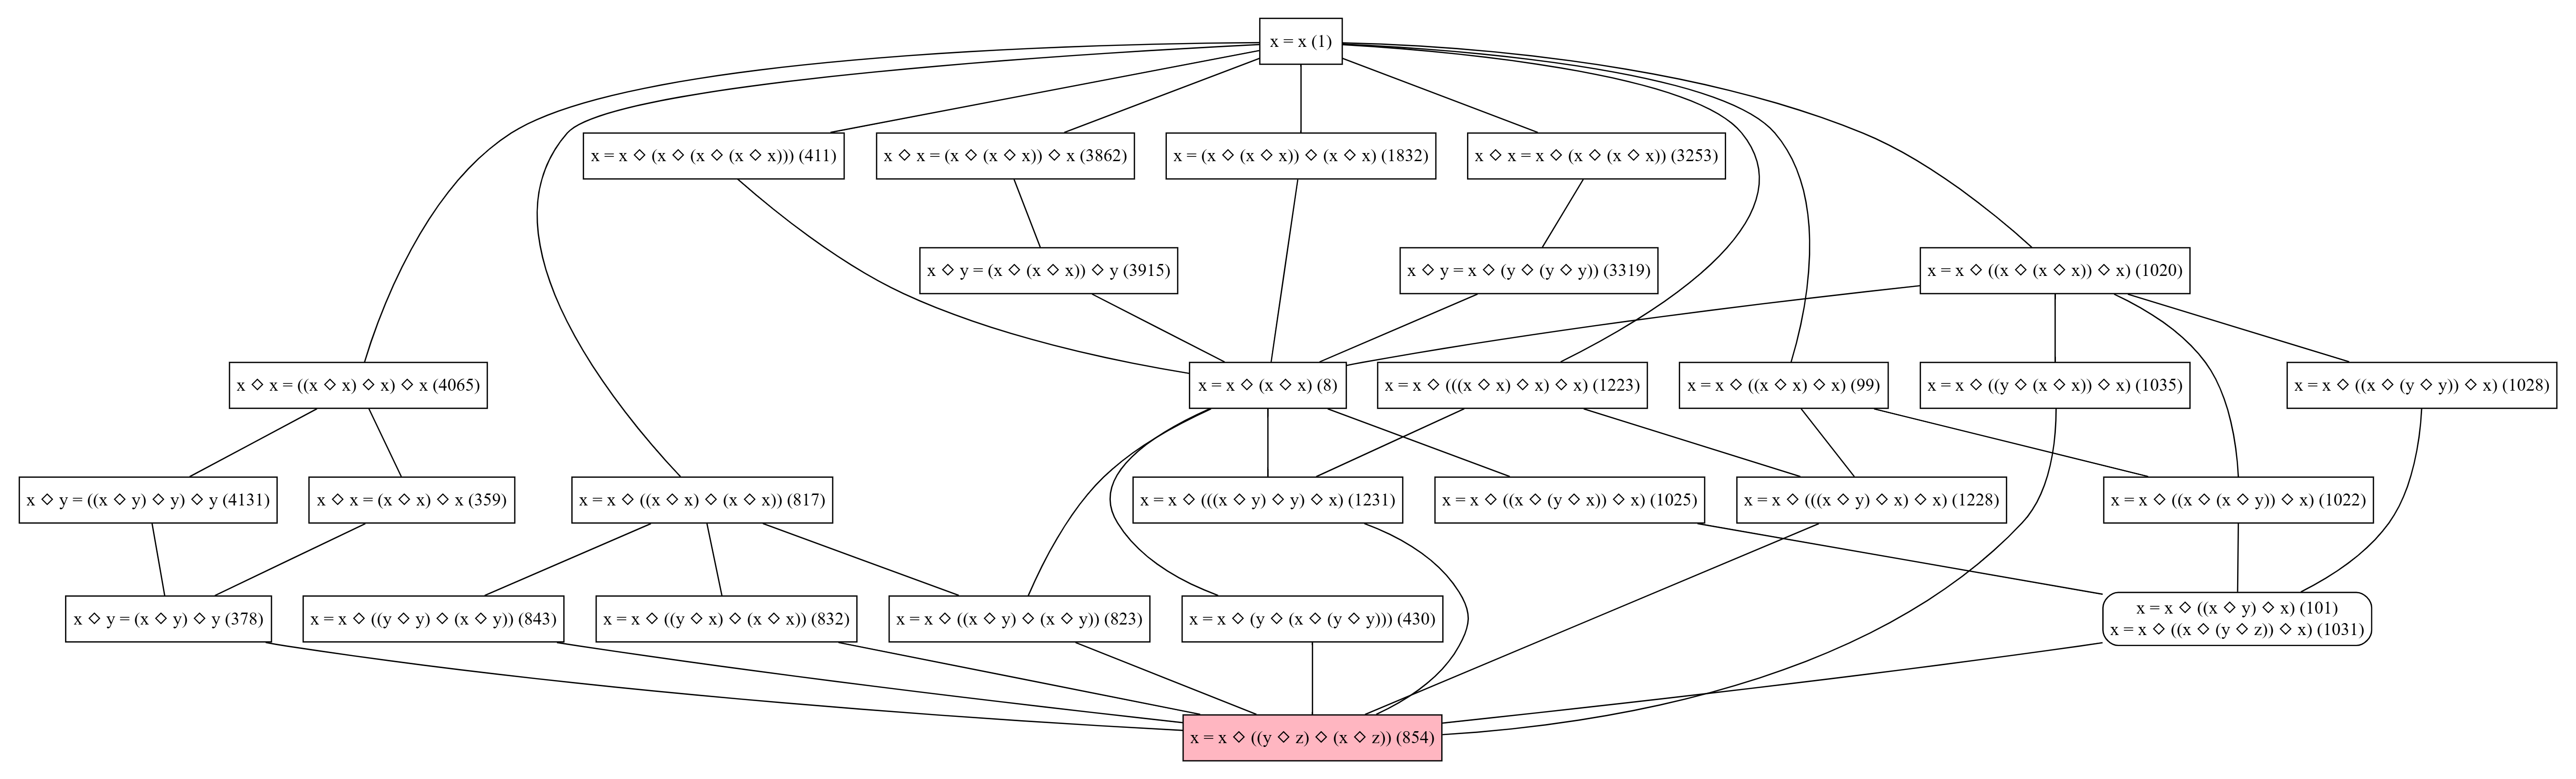
\includegraphics[width=0.85\textwidth]{854.png}
\caption{A Hasse diagram of all the equational laws implied by \Cref{eq854}.  An edge in this diagram indicates that the lower equation implies the higher one. Rounded rectangles indicate groups of equivalent laws.  This graph was produced by the visualization tool \emph{Graphiti}, which was developed for this project.}
\label{fig:854}
\end{figure}


Of the $22033636$ possible implications $E \vdash E'$, $8178279$ (or $37.12\%$) would end up being true. To establish such positive implications $E \vdash E'$, the main techniques used were as follows:

\begin{itemize}
    \item A very small number of positive implications were established and formalized by hand, mostly through direct rewriting of the laws; but this approach would not scale to the full project.
    \item Simple rewriting rules, for instance based on the observation that any law of the form $\x \formaleq f(\y,\z,\dots)$ was necessarily equivalent to the trivial law \Cref{eq2}, could already reduce the size of potential equivalence classes by a significant fraction. We discuss this method in \Cref{rewrite-sec}.
    \item The preorder axioms for $\vdash$, as well as the ``duality'' symmetry of the preorder with respect to replacing a magma operation $x \op y$ with its opposite $x \op^{\mathrm{op}} y \coloneqq y \op x$, can be used to significantly cut down on the number of implications that need to be proven explicitly; ultimately, only $10657$ ($0.05\%$) of the positive implications needed a direct proof.
    \item Automated Theorem Provers (ATP) could be deployed at extremely fast speeds to establish a complete generating set of positive implications; see \Cref{automated-sec}.
\end{itemize}

More challenging were the $13855357$ ($62.88\%$) implications that were false, $E \not \vdash E'$. Here, the range of techniques needed to refute such implications were quite varied.
\begin{itemize}
        \item Syntactic methods, such as observing an ``matching invariant'' of the law $E$ that was not shared by the law $E'$, could be used to obtain some refutations.  For instance, if both sides of $E$ had the same order, but both sides of $E'$ did not, this could be used to syntactically refute $E \vdash E'$.  Similarly, if the law $E$ was confluent, enjoyed a complete rewriting system, or otherwise permitted some understanding of the free magma associated to that law, one could decide the assertions $E \vdash E'$ for all possible laws $E'$, or at least a significant fraction of such laws.  We discuss these methods, and the extent to which they can be automated in \Cref{syntactic-sec}.
        \item Small finite magmas, which can be described explicitly by multiplication tables, could be tested by brute force computations to provide a large number of counterexamples to implications, or by ATP-assisted methods. See \Cref{finite-sec}.
        \item Linear models, in which the magma operation took the form $x \op y = ax + by$ for some (commuting or non-commuting) coefficients $a,b$, allowed for another large class of counterexamples to implications, which could be automatically scanned for either by brute force or by Grobner basis type calculations. See \Cref{linear-sec}.
        \item Translation invariant models, in which the magma operation took the form $x \op y = x + f(y-x)$ on an additive group, or $x \op y = x f(x^{-1} y)$ on a non-commutative group, reduce matters to analyzing certain functional equations; see \Cref{translation-sec}.
        \item Greedy methods, in which either the multiplication table $(x,y) \mapsto x \op y$ or the function $f$ determining a translation-invariant model are iteratively constructed by a greedy algorithm subject to a well-chosen ruleset, were effective in resolving many implications not easily disposed of by preceding methods. See \Cref{greedy-sec}.
        \item Starting with a simple base magma $M$ obeying both $E$ and $E'$, and either enlarging it to a larger magma $M' \supset M$, extending it to a magma $N$ with a projection homomorphism $\pi: N \to M$, or modifying the multiplication table on a small number of values, also proved effective when combined with greedy methods. See \Cref{modify-base}.
        \item To each equation $E$ one can associate a ``twisting semigroup'' $S_E$.  If $S_E$ is larger than $S_{E'}$, then this can often be used to disprove the implication $E \vdash E'$; see \Cref{twisting-sec}.
        \item Some \emph{ad hoc} models based on existing mathematical objects, such as infinite trees, rings of polynomials, or ``Kisielewicz models'' utilizing the prime factorization of the natural numbers, could also handle some otherwise difficult cases.  In some cases, the magma law induced some relevant and familiar structures, such as a directed graph or a partial order, which also helped guide counterexample constructions. See \Cref{adhoc-sec}.
        \item Automated theorem provers were helpful in identifying which simplifying axioms could be added to the magma without jeopardizing the ability to refute the desired implication $E \vdash E'$.
\end{itemize}

\subsection{Extensions}

While the primary objective of the ETP was being completed, some additional related results were generated as spinoffs.  Specifically:
\begin{itemize}
\item In \Cref{finite-sec} we report on a variant of the implication graph of the original set of 4692 equations, in which the magma is required to be finite.
\item In \Cref{order-5} we report on classifying which of the $57882$ distinct laws of order $5$ are equivalent to the singleton law \Cref{eq2}, either with or without the requirement that the magma be finite.
\item In \Cref{higman-neumann} we report on classifying the laws of order $8$ that are equivalent to the Higman-Neumann law \Cref{eq42323216}.
\end{itemize}

\note{Also mention ML stuff, GUI}

\chapter{Selected laws}\label{subgraph-eq}

In this project we study the 4694 laws (up to symmetry and relabeling) of total order at most $4$.

Selected laws of interest are listed below, as well as in \href{https://github.com/teorth/equational_theories/blob/main/equational_theories/Equations/Basic.lean}{this file}.

\begin{definition}[Equation 1]\label{eq1}\lean{Equation1}\leanok\uses{magma-def}  Equation 1 is the law $0 \formaleq 0$ (or the equation $x=x$).
\end{definition}

This is the trivial law, satisfied by all magmas. It is self-dual.


\begin{definition}[Equation 2]\label{eq2}\lean{Equation2}\leanok\uses{magma-def}  Equation 2 is the law $0 \formaleq 1$ (or the equation $x=y$).
\end{definition}

This is the singleton law, satisfied only by the empty and singleton magmas.  It is self-dual.

\begin{definition}[Equation 3]\label{eq3}\lean{Equation3}\leanok\uses{magma-def}  Equation 3 is the law $0 \formaleq 0 \op 0$ (or the equation $x = x \op x$).
\end{definition}

This is the idempotence law.  It is self-dual.

\begin{definition}[Equation 4]\label{eq4}\lean{Equation4}\leanok\uses{magma-def}  Equation 4 is the law $0 \formaleq 0 \op 1$ (or the equation $x = x \op y$).
\end{definition}

This is the left absorption law.

\begin{definition}[Equation 5]\label{eq5}\lean{Equation5}\leanok\uses{magma-def}  Equation 5 is the law $0 \formaleq 1 \op 0$ (or the equation $x = y \op x$).
\end{definition}

This is the right absorption law (the dual of \Cref{eq4}).

\begin{definition}[Equation 6]\label{eq6}\lean{Equation6}\leanok\uses{magma-def}  Equation 6 is the law $0 \formaleq 1 \op 1$ (or the equation $x = y \op y$).
\end{definition}

This law is equivalent to the singleton law.

\begin{definition}[Equation 7]\label{eq7}\lean{Equation7}\leanok\uses{magma-def}  Equation 7 is the law $0 \formaleq 1 \op 2$ (or the equation $x = y \op z$).
\end{definition}

This law is equivalent to the singleton law.

\begin{definition}[Equation 8]\label{eq8}\lean{Equation8}\leanok\uses{magma-def}  Equation 8 is the law $0 \formaleq 0 \op (0 \op 0)$ (or the equation $x = x \op (x \op x)$).
\end{definition}

\begin{definition}[Equation 14]\label{eq14}\lean{Equation14}\leanok\uses{magma-def}  Equation 14 is the law $0 \formaleq  1 \op (0 \op 1)$ (or the equation $x = y \op (x \op y))$.
\end{definition}

Appears in Problem A1 from Putnam 2001.  See \Cref{29_equiv_14}.

\begin{definition}[Equation 16]\label{eq16}\lean{Equation16}\leanok\uses{magma-def}  Equation 16 is the law $0 \formaleq  1 \op (1 \op 0)$ (or the equation $x = y \op (y \op x))$.
\end{definition}

\begin{definition}[Equation 23]\label{eq23}\lean{Equation23}\leanok\uses{magma-def}  Equation 23 is the law $0 \formaleq  (0 \op 0) \op 0$ (or the equation $x = (x \op x) \op x$).
\end{definition}

This is the dual of \Cref{eq8}.

\begin{definition}[Equation 29]\label{eq29}\lean{Equation29}\leanok\uses{magma-def}  Equation 29 is the law $0 \formaleq  (1 \op 0) \op 1$ (or the equation $x = (y \op x) \op y)$.
\end{definition}

Appears in Problem A1 from Putnam 2001.  Dual to \Cref{eq14}.  See \Cref{29_equiv_14}.

\begin{definition}[Equation 38]\label{eq38}\lean{Equation38}\leanok\uses{magma-def}  Equation 38 is the law $0 \op 0  \formaleq  0 \op 1$ (or the equation $x \op x = x \op y$).
\end{definition}

This law asserts that the magma operation is independent of the second argument.

\begin{definition}[Equation 39]\label{eq39}\lean{Equation39}\leanok\uses{magma-def}  Equation 39 is the law $0 \op 0  \formaleq  1 \op 0$ (or the equation $x \op x = y \op x$).
\end{definition}

This law asserts that the magma operation is independent of the first argument (the dual of \Cref{eq38}).

\begin{definition}[Equation 40]\label{eq40}\lean{Equation40}\leanok\uses{magma-def}  Equation 40 is the law $0 \op 0  \formaleq  1 \op 1$ (or the equation $x \op x = y \op y$).
\end{definition}

This law asserts that all squares are constant. It is self-dual.

\begin{definition}[Equation 41]\label{eq41}\lean{Equation41}\leanok\uses{magma-def}  Equation 41 is the law $0 \op 0  \formaleq  1 \op 2$ (or the equation $x \op x = y \op z$).
\end{definition}

This law is equivalent to the constant law, \Cref{eq46}.

\begin{definition}[Equation 42]\label{eq42}\lean{Equation42}\leanok\uses{magma-def}  Equation 42 is the law $0 \op 1  \formaleq  0 \op 2$ (or the equation $x \op y = x \op z$).
\end{definition}

Equivalent to \Cref{eq38}.

\begin{definition}[Equation 43]\label{eq43}\lean{Equation43}\leanok\uses{magma-def}  Equation 43 is the law $0 \op 1  \formaleq  1 \op 0$ (or the equation $x \op y = y \op x$).
\end{definition}

The commutative law. It is self-dual.

\begin{definition}[Equation 45]\label{eq45}\lean{Equation45}\leanok\uses{magma-def}  Equation 45 is the law $0 \op 1  \formaleq  2 \op 1$ (or the equation $x \op y = z \op y$).
\end{definition}

This is the dual of \Cref{eq42}.

\begin{definition}[Equation 46]\label{eq46}\lean{Equation46}\leanok\uses{magma-def}  Equation 46 is the law $0 \op 1  \formaleq  2 \op 3$ (or the equation $x \op y = z \op w$).
\end{definition}

The constant law: all products are constant. It is self-dual.

\begin{definition}[Equation 63]\label{eq63}\lean{Equation63}\leanok\uses{magma-def}  Equation 63 is the law $0 \formaleq 1 \op (0 \op (0 \op 1))$ (or the equation $x = y \op (x \op (x \op y))$).
\end{definition}

The ``Dupont'' law, studied further in Section~\ref{dupont-section}.

\begin{definition}[Equation 65]\label{eq65}\lean{Equation65}\leanok\uses{magma-def}  Equation 65 is the law $0 \formaleq 1 \op (0 \op (1 \op 0))$ (or the equation $x = y \op (x \op (y \op x))$).
\end{definition}

The ``Asterix'' law, studied further in Section~\ref{asterix-section}.

\begin{definition}[Equation 168]\label{eq168}\lean{Equation168}\leanok\uses{magma-def}  Equation 168 is the law $0  \formaleq  (1 \op 0) \op (0 \op 2)$ (or the equation $x = (y \op x) \op (x \op z)$).
\end{definition}

The law of a central groupoid. It is self-dual.

\begin{definition}[Equation 206]\label{eq206}\lean{Equation206}\leanok\uses{magma-def}  Equation 206 is the law $0  \formaleq  (0 \op (0 \op 1)) \op 1$ (or the equation $x = (x \op (x \op y)) \op y$).
\end{definition}

Our project located this law as one member of an ``Austin pair''; see Chapter \ref{infinite-model-chapter}. The infinite counterexample is constructed using the infinite 3-regular tree.

\begin{definition}[Equation 381]\label{eq381}\lean{Equation381}\leanok\uses{magma-def}  Equation 381 is the law $0 \op 1  \formaleq  (0 \op 2) \op 1$ (or the equation $x \op y = (x \op z) \op y$).
\end{definition}

Appears in Putnam 1978, Problem A4, part (b).

\begin{definition}[Equation 387]\label{eq387}\lean{Equation387}\leanok\uses{magma-def}  Equation 387 is the law $0 \op 1  \formaleq  (1 \op 1) \op 0$ (or the equation $x \op y = (y \op y) \op x$).
\end{definition}

Introduced in \href{https://mathoverflow.net/a/450905/766}{MathOverflow}. See \Cref{387_implies_43}

\begin{definition}[Equation 477]\label{eq477}\lean{Equation477}\leanok\uses{magma-def}  Equation 477 is the law $0 \formaleq 1 \op (0 \op (1 \op (1 \op 1)))$ (or the equation $x = y \op (x \op (y \op (y \op y)))$).
\end{definition}

An example of a confluent law; see \Cref{477-confl}.

\begin{definition}[Equation 854]\label{eq854}\lean{Equation953}\leanok\uses{magma-def}  Equation 854 is the law $0 = 0 \op ((1 \op 2) \op (0 \op 2))$ (or the equation $x = x \op ((y \op z) \op (x \op z))$).
\end{definition}

Studied in \Cref{854-chapter}


\begin{definition}[Equation 953]\label{eq953}\lean{Equation953}\leanok\uses{magma-def}  Equation 953 is the law $0 = 1 \op ((2 \op 0) \op (2 \op 2))$ (or the equation $x = y \op ((z \op x) \op (z \op z))$).
\end{definition}

An example of a trivial law; see \Cref{953_equiv_2}.

\begin{definition}[Equation 1485]\label{eq1485}\lean{Equation1491}\leanok\uses{magma-def}  Equation 1485 is the law $0 \formaleq  (1 \op 0) \op (0 \op (2 \op 1))$ (or the equation $x = (y \op x) \op (x \op (z \op y))$).
\end{definition}

The ``Obelix'' law, studied further in Section~\ref{asterix-section}.

\begin{definition}[Equation 1491]\label{eq1491}\lean{Equation1491}\leanok\uses{magma-def}  Equation 1491 is the law $0 \formaleq  (1 \op 0) \op (1 \op (1 \op 0))$ (or the equation $x = (y \op x) \op (y \op (y \op x))$).
\end{definition}

The ``Obelix'' law, studied further in Section~\ref{asterix-section}.

\begin{definition}[Equation 1571]\label{eq1571}\lean{Equation1571}\leanok\uses{magma-def}  Equation 1571 is the law $0 \formaleq  (1 \op 2) \op (1 \op (0 \op 2))$ (or the equation $x = (y \op z) \op (y \op (x \op z))$).
\end{definition}

Introduced in \cite{mendelsohn-padmanabhan}.  As shown in \Cref{1571_impl}, this law characterizes abelian groups of exponent two.

\begin{definition}[Equation 1648]\label{eq1648}\lean{Equation1648}\leanok\uses{magma-def}  Equation 1648 is the law $0 \formaleq  (0 \op 1) \op ((0 \op 1) \op 1)$ (or the equation $x = (x \op y) \op ((x \op y) \op y)$).
\end{definition}

The golden ratio is a coefficient of the linearization of this law.

\begin{definition}[Equation 1657]\label{eq1657}\lean{Equation1657}\leanok\uses{magma-def}  Equation 1657 is the law $0 \formaleq  (0 \op 1) \op ((1 \op 1) \op 0)$ (or the equation $x = (x \op y) \op ((y \op y) \op x)$).
\end{definition}

\begin{definition}[Equation 1659]\label{eq1659}\lean{Equation1659}\leanok\uses{magma-def}  Equation 1659 is the law $0 \formaleq  (0 \op 1) \op ((1 \op 1) \op 2)$ (or the equation $x = (x \op y) \op ((y \op y) \op z)$).
\end{definition}

\begin{definition}[Equation 1661]\label{eq1661}\lean{Equation1661}\leanok\uses{magma-def}  Equation 1661 is the law $0 \formaleq  (0 \op 1) \op ((1 \op 2) \op 1)$ (or the equation $x = (x \op y) \op ((y \op z) \op y)$).
\end{definition}

These two laws admit infinite models on the natural numbers arising from the modified base model construction. See Section~\ref{infinite-examples-section}.

\begin{definition}[Equation 1689]\label{eq1689}\lean{Equation1689}\leanok\uses{magma-def}  Equation 1689 is the law $0 \formaleq  (1 \op 0) \op ((0 \op 2) \op 2)$ (or the equation $x = (y \op x) \op ((x \op z) \op z)$).
\end{definition}

Mentioned in \cite{Kisielewicz2}.  See \Cref{1689_equiv_2}.

\begin{definition}[Equation 1701]\label{eq1701}\lean{Equation1701}\leanok\uses{magma-def}  Equation 1701 is the law $0 \formaleq  (1 \op x) \op ((2 \op 0) \op 0)$ (or the equation $x = (y \op x) \op ((z \op x) \op x)$).
\end{definition}

This law admits infinite models on the natural numbers arising from the modified base model construction. See Section~\ref{infinite-examples-section}.

\begin{definition}[Equation 2662]\label{eq2662}\lean{Equation2662}\leanok\uses{magma-def}  Equation 2662 is the law $0 \formaleq  ((0 \op 1) \op (0 \op 1)) \op 0$ (or the equation $x = ((x \op y) \op (x \op y)) \op x$).
\end{definition}

Appears in \cite{mendelsohn-padmanabhan}.

\begin{definition}[Equation 3167]\label{eq3167}\lean{Equation3167}\leanok\uses{magma-def}  Equation 3167 is the law $0 \formaleq  (((1 \op 1) \op 2) \op 2) \op 0$ (or the equation $x = (((y \op y) \op z) \op z) \op x$).
\end{definition}


\begin{definition}[Equation 3588]
  \label{eq3588}\lean{Equation3588}\leanok\uses{magma-def}
  Equation 3588 is the law $0 \op 1 \formaleq 2 \op ((0 \op 1) \op 2)$ (or the equation $x \op y = z \op ((x \op y) \op z)$).
\end{definition}

Our project located this law as one member of an ``Austin pair''; see Chapter \ref{infinite-model-chapter}.

\begin{definition}[Equation 3722]\label{eq3722}\lean{Equation3722}\leanok\uses{magma-def}  Equation 3722 is the law $0 \op 1  \formaleq  (0 \op 1) \op (0 \op 1)$ (or the equation $x \op y = (x \op y) \op (x \op y)$).
\end{definition}

Appears in Putnam 1978, Problem A4, part (a).  It is self-dual.

\begin{definition}[Equation 3744]\label{eq3744}\lean{Equation3744}\leanok\uses{magma-def}  Equation 3744 is the law $0 \op 1  \formaleq  (0 \op 2) \op (3 \op 1)$ (or the equation $x \op y = (x \op z) \op (w \op y)$).
\end{definition}

This law is called a ``bypass operation'' in Putnam 1978, Problem A4. It is self-dual.  See \Cref{3744_implies_3722_381}.

\begin{definition}[Equation 3994]
  \label{eq3994}\uses{magma-def}
  Equation 3994 is the law $0 \op 1 \formaleq (2 \op (0 \op 1)) \op 2$ (or the equation $x \op y = (z \op (x \op y)) \op z$).
\end{definition}

Our project located this law as one member of an ``Austin pair''; see Chapter \ref{infinite-model-chapter}.

\begin{definition}[Equation 4315]\label{eq4315}\lean{Equation4315}\leanok\uses{magma-def}  Equation 4315 is the law $0 \op (1 \op 0)  \formaleq  0 \op (1 \op 2)$ (or the equation $x \op (y \op x) = x \op (y \op z)$).
\end{definition}

\begin{definition}[Equation 4512]\label{eq4512}\lean{Equation4512}\leanok\uses{magma-def}  Equation 4512 is the law $0 \op (1 \op 2)  \formaleq  (0 \op 1) \op 2$ (or the equation $x \op (y \op z) = (x \op y) \op z$).
\end{definition}

The associative law. It is self-dual.

\begin{definition}[Equation 4513]\label{eq4513}\lean{Equation4513}\leanok\uses{magma-def}  Equation 4513 is the law $0 \op (1 \op 2)  \formaleq  (0 \op 1) \op 3$ (or the equation $x \op (y \op z) = (x \op y) \op w$).
\end{definition}

\begin{definition}[Equation 4522]\label{eq4522}\lean{Equation4522}\leanok\uses{magma-def}  Equation 4522 is the law $0 \op (1 \op 2)  \formaleq  (0 \op 3) \op 4$ (or the equation $x \op (y \op z) = (x \op w) \op u$).
\end{definition}

Dual to \Cref{eq4579}.

\begin{definition}[Equation 4564]\label{eq4564}\lean{Equation4564}\leanok\uses{magma-def}  Equation 4564 is the law $0 \op (1 \op 2)  \formaleq  (3 \op 1) \op 2$ (or the equation $x \op (y \op z) = (w \op y) \op z$).
\end{definition}

Dual to \Cref{eq4513}.

\begin{definition}[Equation 4579]\label{eq4579}\lean{Equation4579}\leanok\uses{magma-def}  Equation 4579 is the law $0 \op (1 \op 2)  \formaleq  (3 \op 4) \op 2$ (or the equation $x \op (y \op z) = (w \op u) \op z$).
\end{definition}

Dual to \Cref{eq4522}.

\begin{definition}[Equation 4582]\label{eq4582}\lean{Equation4582}\leanok\uses{magma-def}  Equation 4582 is the law $0 \op (1 \op 2)  \formaleq  (3 \op 4) \op 5$ (or the equation $x \op (y \op z) = (w \op u) \op v$).
\end{definition}

This law asserts that all triple constants (regardless of bracketing) are constant.

\section{Equations of order greater than \texorpdfstring{$4$}{4}}

We note some selected laws of order more than $5$, which are used in some later chapters of the blueprint.

\begin{definition}[Equation 5093]
  \label{eq5093}\uses{magma-def}\lean{Equation5093}\leanok
  Equation 5093 is the law $0  \formaleq 1 \op (1 \op (1 \op (0 \op (2 \op 1))))$ (or the equation $x = y \op (y \op (y \op (x \op (z \op y))))$).
\end{definition}

This law of order $5$ was mentioned in \cite{Kisielewicz2}.  See \Cref{5093-nontrivial}.

\begin{definition}[Equation 26302]
  \label{eq26302}\uses{magma-def}
  Equation 26302 is the law $0  \formaleq (1 \op ((2 \op 0) \op 3)) \op (0 \op 3)$ (or the equation $x = (y \op ((z \op x) \op w)) \op (x \op w)$).
\end{definition}

A law that characterizes natural central groupoids; see \Cref{natural-central-groupoid}.

\begin{definition}[Equation 28770]
  \label{eq28770}\uses{magma-def}\lean{Equation28770}\leanok
  Equation 28770 is the law $0  \formaleq  (((1 \op 1) \op 1) \op 0) \op (1 \op 2)$ (or the equation $x = (((y \op y) \op y) \op x) \op (y \op z)$).
\end{definition}

This law of order $5$ was introduced by Kisielewicz \cite{Kisielewicz}. See \Cref{kis-thm2}.

\begin{definition}[Equation 345169]
  \label{eq345169}\uses{magma-def}
  Equation 345169 is the law $0  \formaleq  (1 \op ((0 \op 1) \op 1)) \op (0 \op (2 \op 1))$ (or the equation $x = (y \op ((x \op y) \op y)) \op (x \op (z \op y))$).
\end{definition}

This law of order $6$ was shown in \cite{mccune_et_al} to characterize the Sheffer stroke in a boolean algebra; see \Cref{sheffer}.

\begin{definition}[Equation 374794]
  \lean{Equation374794}\leanok
  \label{eq374794}\uses{magma-def}
  Equation 374794 is the law $0  \formaleq  (((1 \op 1) \op 1) \op 0) \op ((1 \op 1) \op 2)$ (or the equation $x = (((y \op y) \op y) \op x) \op ((y \op y) \op z)$).
\end{definition}

This law of order $6$ was introduced by Kisielewicz \cite{Kisielewicz}; see \Cref{kis-thm}.

\chapter{General implications}

We will be interested in seeing which laws imply which other laws, in the sense that magmas obeying the former law automatically obey the latter.  We will also be interested in \emph{anti-implications} showing that one law does \emph{not} imply another, by producing examples of magmas that obey the former law but not the latter. Here is a formal definition.

\begin{definition}[Implication]\label{impl}\uses{models-def}  A law $E$ is said to \emph{imply} another law $E'$ if $\{E\} \models E'$, or equivalently:
  $$ G \models w  \formaleq  w' \implies G \models w''  \formaleq  w''' \hbox{ for all magmas } G$$
Two laws are said to be \emph{equivalent} if they imply each other.
\end{definition}

\begin{lemma}[Pre-order]\leanok\label{pre-order}\uses{impl}  If we define $E \leq E'$ if $E$ implies $E'$, then this is a pre-order on the set of laws, and equivalence is an equivalence relation.
\end{lemma}

Note that we view the stronger law as less than or equal to the weaker law.  This is because the class of magmas that obey the stronger law is a subset of the class of magmas that obey the weaker law.  It is also consistent with the conventions of Lean's Mathlib.

\begin{proof}\leanok Trivial.
\end{proof}

Implications between the laws from Chapter \ref{subgraph-eq} are depicted in Figure \ref{fig:implications}.

\begin{figure}
  \centering
  \includegraphics[width=0.5\linewidth]{../../images/implications.png}
  \caption{Implications between the above equations, displayed as a Hasse diagram.}
  \label{fig:implications}
\end{figure}


\begin{lemma}[Maximal element]\label{maximal}\uses{pre-order}  The law $0  \formaleq  0$ is the maximal element in this pre-order.
\end{lemma}

\begin{proof} Trivial.
\end{proof}

\begin{lemma}[Minimal element]\label{minimal}\uses{pre-order}  The law $0  \formaleq  1$ is the minimal element in this pre-order.
\end{lemma}

\begin{proof} Trivial.
\end{proof}

Every magma $G$ has a \emph{reversal} $G^{\mathrm{op}}$, formed by by replacing the magma operation $\circ$ with its opposite $\circ^{\mathrm{op}}:(x,y) \mapsto y \circ x$. There is a natural isomorphism between these magmas, which induces an involution $w \mapsto w^{\mathrm{op}}$ on words $w \in M_X$.  Every law $w  \formaleq  w'$ then has a \emph{dual} $w^{\mathrm{op}}  \formaleq  (w')^{\mathrm{op}}$.

For instance, the dual of the law $0 \circ 1 = 0 \circ 2$ is $1 \circ 0 = 2 \circ 0$, which after relabeling is $0 \circ 1 = 2 \circ 1$.  A list of equations and their duals can be found \href{https://github.com/teorth/equational_theories/blob/main/data/dual_equations.md}{here}.  Of the 4694 equations under consideration, 84 are self-dual, leaving 2305 pairs of dual equations.

The pre-ordering on laws has a duality symmetry:

\begin{lemma}[Duality of laws]\label{duality}\uses{pre-order}  If $w  \formaleq  w'$ implies $w''  \formaleq  w'''$, then $w^{\mathrm{op}}  \formaleq  (w')^{\mathrm{op}}$ implies $w''^{\mathrm{op}}  \formaleq  (w''')^{\mathrm{op}}$.
\end{lemma}

\begin{proof} This follows from the fact that a magma $G$ satisfies a law $w  \formaleq  w'$ if and only if $G^{\mathrm{op}}$ satisfies $w^{\mathrm{op}}  \formaleq  (w')^{\mathrm{op}}$.
\end{proof}

Some equational laws can be ``diagonalized'':

\begin{theorem}[Diagonalization]\label{diag}  An equational law of the form
  \begin{equation}\label{prediag} F(x_1,\dots,x_n) = G(y_1,\dots,y_m),
  \end{equation}
  where $x_1,\dots,x_n$ and $y_1,\dots,y_m$ are distinct elements of the alphabet, implies the diagonalized law
$$ F(x_1,\dots,x_n) = F(x'_1,\dots,x'_n).$$
where $x'_1,\dots,x'_n$ are distinct from $x_1,\dots,x_n$
In particular, if $G(y_1,\dots,y_m)$ can be viewed as a specialization of $F(x'_1,\dots,x'_n)$, then these two laws are equivalent.
\end{theorem}

\begin{proof}  From two applications of \eqref{prediag} one has
$$ F(x_1,\dots,x_n) = G(y_1,\dots,y_m)$$
and
$$ F(x'_1,\dots,x'_n) = G(y_1,\dots,y_m)$$
whence the claim.
\end{proof}

Thus for instance, Definition \ref{eq7} is equivalent to Definition \ref{eq2}.

\begin{theorem}[Laws implied by the constant law]\label{constant-impl}\uses{impl,eq46}  If $w, w'$ each have order at least one, then the law $w \formaleq w'$ is implied by the constant law (Definition \ref{eq46}).  If exactly one of $w, w'$ has order zero, and the law $w \formaleq w'$ is not implied by the constant law.
\end{theorem}

\begin{proof} Routine.
\end{proof}

\begin{theorem}[Criterion for implication]\label{variable-impl}\uses{impl}\lean{Law.MagmaLaw.SameCount.derive}\leanok  If $w \formaleq w'$ is such that every variable appears the same number of times in both $w$ and $w'$, and $w \formaleq w'$ implies another law $w'' \formaleq w'''$, then every variable appears the same number of times in both $w''$ and $w'''$.
\end{theorem}

\begin{proof} Consider the magma $\mathrm{MS}$ of multisets over an arbitrary set $A$ (which can be seen as finitely suported maps $A\rightarrow \N$), with the multiset addition law $+$.  By hypothesis, this magma obeys $w \formaleq w'$, and hence $w'' \formaleq w'''$, giving the claim by comparing the orders of the elements of $A$ appearing in $w''$ and $w'''$ in this magma.
\end{proof}

\chapter{Implications between selected laws}\label{implications-chapter}

We collect here some notable implications between the the selected laws in \Cref{subgraph-eq}.   By \Cref{sound-complete}, every implication can basically be established by a finite number of rewrites.  In most cases, the sequence of rewrites is quite straightforward, and the implication is very easy, but we record some less obvious examples.

\begin{theorem}[387 implies 43]\label{387_implies_43}\uses{eq387,eq43}\lean{Subgraph.Equation387_implies_Equation43}\leanok  \Cref{eq387} implies \Cref{eq43}.
\end{theorem}

\begin{proof}\leanok (From \href{https://mathoverflow.net/a/450905/766}{MathOverflow}).
  By \Cref{eq387}, one has the law
\begin{equation}\label{387-again}
  (x \op x) \op y = y \op x.
\end{equation}
Specializing to $y=x \op x$, we conclude
$$(x \op x) \op (x \op x) = (x \op x) \op x$$
and hence by another application of \Cref{eq387} we see that $x \op x$ is idempotent:
\begin{equation}\label{idem}
  (x \op x) \op (x \op x) = x \op x.
\end{equation}
Now, replacing $x$ by $x \op x$ in \Cref{387-again} and then using \Cref{idem} we see that
$$ (x \op x) \op y = y \op (x \op x)$$
so in particular $x \op x$ commutes with $y \op y$:
\begin{equation}\label{op-idem} (x \op x) \op (y \op y) = (y \op y) \op (x \op x).
\end{equation}
Also, from two applications of \Cref{387-again} one has
$$(x \op x) \op (y \op y) = (y \op y) \op x = x \op y.$$
Thus \Cref{op-idem} simplifies to $x \op y = y \op x$, which is \Cref{eq43}.
\end{proof}

\begin{theorem}[29 equivalent to 14]\label{29_equiv_14} \uses{eq29,eq14}\lean{Subgraph.Equation29_implies_Equation14}\leanok  \Cref{eq29} is equivalent to \Cref{eq14}.
\end{theorem}

This result was posed as Problem A1 from Putnam 2001.

\begin{proof}\leanok\uses{duality} By \Cref{duality} it suffices to show that \Cref{eq29} implies \Cref{eq14}.  From \Cref{eq29} one has
  $$ x = ((x \op y) \op x) \op (x \op y)$$
  and also
  $$ y = (x \op y) \op x$$
  giving $x = y \op (x \op y)$, which is \Cref{eq14}.
\end{proof}

\begin{theorem}[14 implies 29]\label{14_implies_29} \uses{eq29,eq14}\lean{Subgraph.Equation14_implies_Equation29}\leanok  \Cref{eq14} implies \Cref{eq29}.
\end{theorem}

This result was posed as Problem A1 from Putnam 2001.

\begin{proof}\leanok
\end{proof}

The following result was Problem A4 on Putnam 1978.

\begin{theorem}[3744 implies 3722, 381]\label{3744_implies_3722_381}\uses{eq3744, eq3722, eq381}\lean{Subgraph.Equation3744_implies_Equation3722, Subgraph.Equation3744_implies_Equation381}\leanok \Cref{eq3744} implies \Cref{eq3722} and \Cref{eq381}.
\end{theorem}

\begin{proof}\leanok By hypothesis, one has
$$x \op y = (x \op z) \op (w \op y)
  $$
for all $x,y,z,w$.  Various specializations of this give
\begin{align}
 x \op y &= (x \op z) \op (y \op y) \label{381-1} \\
 x \op z &= (x \op z) \op (x \op z) \label{381-2} \\
(x \op z) \op y &= ((x \op z) \op (x \op z)) \op (y \op y) \label{381-3}.
\end{align}
\Cref{381-2} gives \Cref{eq3722}, while \Cref{381-1}, \Cref{381-2}, \Cref{381-3} gives
$$ x \op y = (x\op z) \op y$$
which is \Cref{eq381}.
\end{proof}

\begin{theorem}[1689 is equivalent to 2]\label{1689_equiv_2}\uses{eq1689, eq2}\lean{Subgraph.Equation1689_implies_Equation2, Subgraph.Equation2_implies_Equation1689}\leanok \Cref{eq1689} is equivalent to \Cref{eq2}.
\end{theorem}


\begin{proof}\leanok  The implication of \Cref{eq1689} from \Cref{eq2} is trivial.  The converse is a surprisingly long chain of implications; see pages 326--327 of \cite{Kisielewicz2}.  The initial law
$$ x = (y \op x) \op ((x \op z) \op z)$$
is used to obtain, in turn,
$$ x \op ((((x \op y) \op y) \op z) \op z) = (x \op y) \op y,$$
$$(x \op (y \op z)) \op (z \op ((z \op w) \op w)) = y \op z,$$
$$x \op (y \op ((y \op z) \op z)) = (x \op y) \op y,$$
$$((x \op (y \op z)) \op z) \op z = y \op z,$$
$$(x \op (y \op (z \op w))) \op (z \op w) = y \op (z \op w),$$
$$(x \op (y \op z)) \op (y \op z) = x \op (y \op z),$$
$$((x \op y) \op ((y \op z) \op z)) \op ((y \op z) \op z) = y,$$
$$((x \op y) \op ((y \op z) \op z)) \op ((y \op z) \op z) = ((x \op ((x \op y) \op ((y \op z) \op z))) \op ((y \op z) \op z)) \op ((y \op z) \op z),$$
$$ x \op ((x \op y) \op y) = x,$$
$$ x \op (x \op (y \op z)) = x,$$
$$ (x \op y) \op y = x \op y,$$
$$ (x \op x) \op x = x,$$
$$ (x \op y) \op y = y,$$
$$ x \op y = y.$$
\end{proof}

The following result was established in \cite{mendelsohn-padmanabhan}.

\begin{theorem}[Consequences of 1571]\label{1571_impl}\uses{eq1571, eq2662, eq40, eq23, eq8, eq16, eq14, eq43, eq4512}\lean{Subgraph.Equation1571_implies_Equation2662, Subgraph.Equation1571_implies_Equation40, Subgraph.Equation1571_implies_Equation23,Subgraph.Equation1571_implies_Equation8, Subgraph.Equation1571_implies_Equation16, Subgraph.Equation1571_implies_Equation43, Subgraph.Equation1571_implies_Equation4512}\leanok  Magmas obeying \Cref{eq1571} also obey \Cref{eq2662}, \Cref{eq40}, \Cref{eq23}, \Cref{eq8}, \Cref{eq16}, \Cref{eq14}, \Cref{eq43}, and \Cref{eq4512}, and are in fact abelian groups of exponent two.  Conversely, all abelian groups of exponent two obey \Cref{eq1571}.
\end{theorem}

\begin{proof}\leanok  Suppose that a magma $G$ obeys \Cref{eq1571}, thus
\begin{equation}\label{1571-again}
 x = (y \op z) \op (y \op (x \op z)).
\end{equation}
$$ x = ((x \op y) \op (x \op y)) \op ((x \op y) \op (x \op (x \op y)))$$
and
$$ x = (x \op y) \op (x \op (x \op y))$$
whence
$$x = ((x \op y) \op (x \op y)) \op x$$
which is \Cref{eq2662}.  This gives
$$y = ((y \op z) \op (y \op z)) \op y$$
while from \Cref{1571-again} one has
$$ (y \op z) \op (y \op z) = (x \op y) \op (x \op ((y \op z) \op (y \op z) \op y))$$
whence
$$ (x \op y) \op (x \op y) = (y \op z) \op (y \op z).$$
This implies that $(x \op y) \op (x \op y)$ does not depend on $x$, or on $y$, hence is equal to some constant $e$:
$$ (x \op y) \op (x \op y) = e.$$
From \Cref{1571-again} the magma operation is surjective, hence
\begin{equation}\label{xxe} x \op x = e
\end{equation}
which gives \Cref{eq40}.  Applying \Cref{1571-again} with $x=y=z$ we conclude
$$ x = e \op (x \op e)$$
while if we instead take $y=z=e$ we have
$$ x = e \op (e \op (x \op e))$$
hence
$$ x = e \op x$$
and then also
$$ x = x \op e$$
from which we readily conclude \Cref{eq23}, \Cref{eq8}; thus $e$ is an identity element.  From \Cref{1571-again} with $z=e$ we now have
\begin{equation}\label{16-again}
 x = y \op (y \op x)
\end{equation}
which is \Cref{eq16}. If instead we take $y=e$ we have
\begin{equation}\label{14-again}
  x = z \op (x \op z)
\end{equation}
which is \Cref{eq14}.  So if we substitute $z = x \op y$ and use \Cref{16-again} we obtain
$$ x = (x \op y) \op y$$
and hence
$$ y \op x = y \op ((x \op y) \op y) = x \op y$$
thanks to \Cref{14-again}.  This gives \Cref{eq43}, thus $G$ is now commutative.  From \Cref{1571-again} once more one has
$$x \op (y \op z) = (y \op x) \op (z \op ((x \op (y \op z)) \op x))$$
which one can simplify using commutativity and \Cref{16-again} (or \Cref{14-again}) to eventually obtain
$$x \op (y \op z) = (x \op y) \op z$$
which is \Cref{eq4512}.  $G$ is now commutative and associative, and every element is its own inverse and of exponent $2$, hence is an abelian group thanks to \Cref{xxe}, so $G$ is an abelian group of exponent $2$ as claimed.  The converse is easily verified.
\end{proof}

\begin{theorem}[953 is equivalent to 2]\label{953_equiv_2}\uses{eq953, eq2}\lean{Subgraph.Equation953_implies_Equation2}\leanok  \Cref{eq953} is equivalent to \Cref{eq2}.
\end{theorem}

\begin{proof}\leanok  It suffices to show that \Cref{eq953} implies \Cref{eq2}.  Pick an element $0$ of $G$ and define $1 = 0 \op 0$ and $2 = 1 \op 1$ (we do not require $0,1,2$ to be distinct).
From \Cref{eq953} with $x=z=0$ we have
$$ 0 = y \op 2.$$
If we then apply \Cref{eq953} with $z=1$ we conclude that
$$ x = y \op 0$$
for all $x,y$, from which one concludes $x=x'$ for any $x,x' \in G$, giving \Cref{eq2}.
\end{proof}


\begin{theorem}[Sheffer stroke axiom]\label{sheffer}\uses{eq345169}\lean{Sheffer.Equation345169_is_Boolean}\leanok  Definition \Cref{eq345169}
axiomatizes the Sheffer stroke operation $x \op y = \overline{xy}$ in a Boolean algebra.
\end{theorem}

\begin{proof}\leanok
See \cite{mccune_et_al}.  In fact this is the shortest law with this property.

A sketch of proof follows.  One can easily verify that the Sheffer stroke operation obeys this law.  Conversely, if this law holds, then automated theorem provers can show that the three Sheffer axioms
$$ (x \op x) \op (x \op x)  = x$$
$$ x \op (y \op (y \op y)) = x \op x$$
$$ (x \op (y \op z)) \op (x \op (y \op z)) = ((y \op y) \op x) \op ((z \op z) \op x)$$
are satisfied.  A classical result of Sheffer \cite{sheffer} then allows one to conclude.
\end{proof}

A \emph{natural central groupoid} is, up to isomorphism, a magma with carrier $S \times S$ for some set $S$ and operation
$$ (a,b) \op (c,d) = (b,c).$$
These are examples of central groupoids (\Cref{eq168}).

\begin{theorem}[Natural central groupoid axiom]\label{natural-central-groupoid}\uses{eq26302} \Cref{eq26302} characterizes natural central groupoids.
\end{theorem}

\begin{proof}
  See \cite[Theorem 5]{knuth}.  The proof is quite lengthy; a sketch is as follows. It is easy to see that natural central groupoids obey \Cref{eq26302}.  Conversely, if this law holds, then
\begin{align*}
  (y \op z) \op (z \op w) &= (( x \op ((w \op (y \op z)) \op w)) \op ((y \op z) \op w)) \op (z \op w)\\
  &= z
\end{align*}
so we have a central groupoid.  Setting $y = (t \op t) \op t$, $z = t \op (t \op t)$, $w = t \op t$ in \Cref{eq26302} we also obtain
$$ (x \op t) \op t = (t \op t) \op t.$$
Using the notation
$$ x^{(1)} := (x \op x) \op x, \quad x^{(2)} := x \op (x \op x)$$
we then have
\begin{align*}
  x \op t &= ((x \op x) \op (x \op t)) \op ((x \op t) \op t) \\
  &= x \op t^{(1)}.
\end{align*}
A lengthy computer-assisted argument then gave the dual identity
$$ t^{(2)} \op x = t \op x$$
Together, these give
$$ x^{(2)} \op y^{(1)} = x \op y.$$
Multiplying on the left by $x = x^{(1)}\op x^{(2)}$, one can conclude that
$$ x^{(2)} = x \op (x \op y).$$
One then has
\begin{align*}
  (x \op y)^{(1)} &= ((y \op x) \op (x \op y)) \op (x \op y) \\
&= x \op (x \op y) \\
&= x^{(2)}
\end{align*}
and a similar argument gives
$$ (x \op y)^{(2)} = y^{(1)}.$$
Since $(x \op x)^{(1)} = x^{(2)}$ and $(x \op x)^{(2)} = x^{(1)}$, we conclude that $x^{(1)}$ and $x^{(2)}$ are idempotent.  Since $x = x^{(1)} \op x^{(2)}$, we see that every $x$ is the product of two idempotents.  One can show that this representation is unique, and gives a canonical identification with a natural central groupoid.
\end{proof}

\chapter{Selected magmas}

Each magma can be used to establish anti-implications: if $\Gamma$ is the set of all laws obeyed by a magma $G$, then we have $\not E \leq E'$ whenever $E \in \Gamma$ and $E' \not \in \Gamma$.  Large numbers of implications can already be obtained from

\begin{itemize}
  \item All magmas of order at most $4$, up to isomorphism (of which there are $178,985,294$);
  \item All commutative magmas of order $5$, up to isomorphism {\bf determine their count};
  \item Cyclic groups $\Z/N\Z$ with $2 \leq N \leq 12$ and $x \circ y = ax^2+bxy+cy^2+dx+ey$ for randomly chosen $a,b,c,d,e$.
\end{itemize}


Some other magmas have been used to establish counterexamples:
\begin{itemize}
  \item The cyclic group $\Z/6\Z$ with the addition law.
  \item The natural numbers with law $x \circ y = x+1$.
  \item The natural numbers with law $x \circ y = xy+1$.
  \item The reals with $x \circ y = (x+y)/2$.
  \item The natural numbers with $x \circ x$ equal to $x$ when $x=y$ and $x+1$ otherwise.
\end{itemize}

\input{chapter/constant.tex}
\input{chapter/simple_rewrites.tex}
\chapter{Trivial auto-generated theorems}

\href{https://github.com/teorth/equational_theories/tree/main/equational_theories/Generated/TrivialBruteforce}{Approximately 4.5m transitive implications were proven by a transitive reduction of about 15k theorems}. Most of these implications were derived from being the first automated run to connect the largest equivalence classes, hence creating a large set of transitively closed implications.

Scripts generated theorems to try simple combinations of equation rewrites to reach the desired goal for every unknown implication. The generated proof scripts were run with lean and the successful theorems were extracted. An example of the types of generated rewrites that were tested:

\begin{verbatim}
  repeat intro
  apply
\end{verbatim}

\begin{verbatim}
  repeat intro
  try { rw [<-h] }
  try { rw [<-h, <-h] }
  try { rw [<-h, <-h, <-h] }
  try { rw [<-h, <-h, <-h, <-h] }
  try { rw [<-h, <-h, <-h, <-h, <-h] }
  repeat rw [h]
\end{verbatim}

\begin{verbatim}
  repeat intro
  try {
    nth_rewrite 1 [h]
    try { rw [h] }
    try { rw [<-h] }
  }
  try {
    nth_rewrite 2 [h]
    try { rw [h] }
    try { rw [<-h] }
  }
  try {
    nth_rewrite 3 [h]
    try { rw [h] }
    try { rw [<-h] }
  }
  try {
    nth_rewrite 4 [h]
    try { rw [h] }
    try { rw [<-h] }
  }
  try {
    nth_rewrite 1 [h]
    nth_rewrite 1 [h]
    try { rw [h] }
    try { rw [<-h] }
  }
  ...
\end{verbatim}

\input{chapter/all_small_magmas.tex}
\chapter{Equation Search}

\href{https://github.com/teorth/equational_theories/tree/main/equational_theories/Generated/EquationSearch}{Approximately ~500k transitive implications were proven by a custom tool leveraging the implication graph}. After previous brute force had derived many implications expressible as a small number of rewrites, this equation search leveraged the implication graph to search further. It began at a hypothesis, and then attempted to perform substitutions by equations it transitively implied. Due to it's naive implementation, it can not perform all forms of substutions, it is limited to substutions that match the exact text of another equation. This search method benefits from being able to start from a hypothesis and can search for any number of goals, rather than having to search the combined space of all possible hypotheses and goals, and can 'reach' farther positions in the search graph than simple rewriting alone.

An example proof illustrates the logic it uses:

\begin{verbatim}
  have eq3315 (x y : G) : x * y = x * (y * (x * x)) := by
    apply Apply.Equation12_implies_Equation11 at h
    apply RewriteHypothesis.Equation11_implies_Equation3323 at h
    apply Apply.Equation3323_implies_Equation3315 at h
    apply h
  have eq52 (x y : G) : x = x * (y * (x * x)) := by
    apply Apply.Equation12_implies_Equation61 at h
    apply Apply.Equation61_implies_Equation54 at h
    apply Apply.Equation54_implies_Equation52 at h
    apply h
  repeat intro
  nth_rewrite 1 [eq3315]
  nth_rewrite 1 [← eq52]
  apply h
  repeat assumption
\end{verbatim}


\bibliographystyle{plain} % We choose the "plain" reference style
\bibliography{references}
